\documentclass{article}

\usepackage[letterpaper, portrait, margin=1in]{geometry}

\usepackage{amsmath, amsfonts, amsthm, amssymb}
\usepackage{graphicx, float}
\usepackage{mathtools}
\usepackage{siunitx}
\usepackage{esdiff}
\usepackage{titlesec}

%opening
\title{Problem Set \#32}
\author{Jayden Li}

\begin{document}

\maketitle

\linespread{1.25}
\fontsize{12pt}{12pt}\selectfont

\section*{Problem 1}
\begin{itemize}

\item[(a, b, d)]
(e) should be corrected to (d)
\begin{figure}[h]
    \centering
    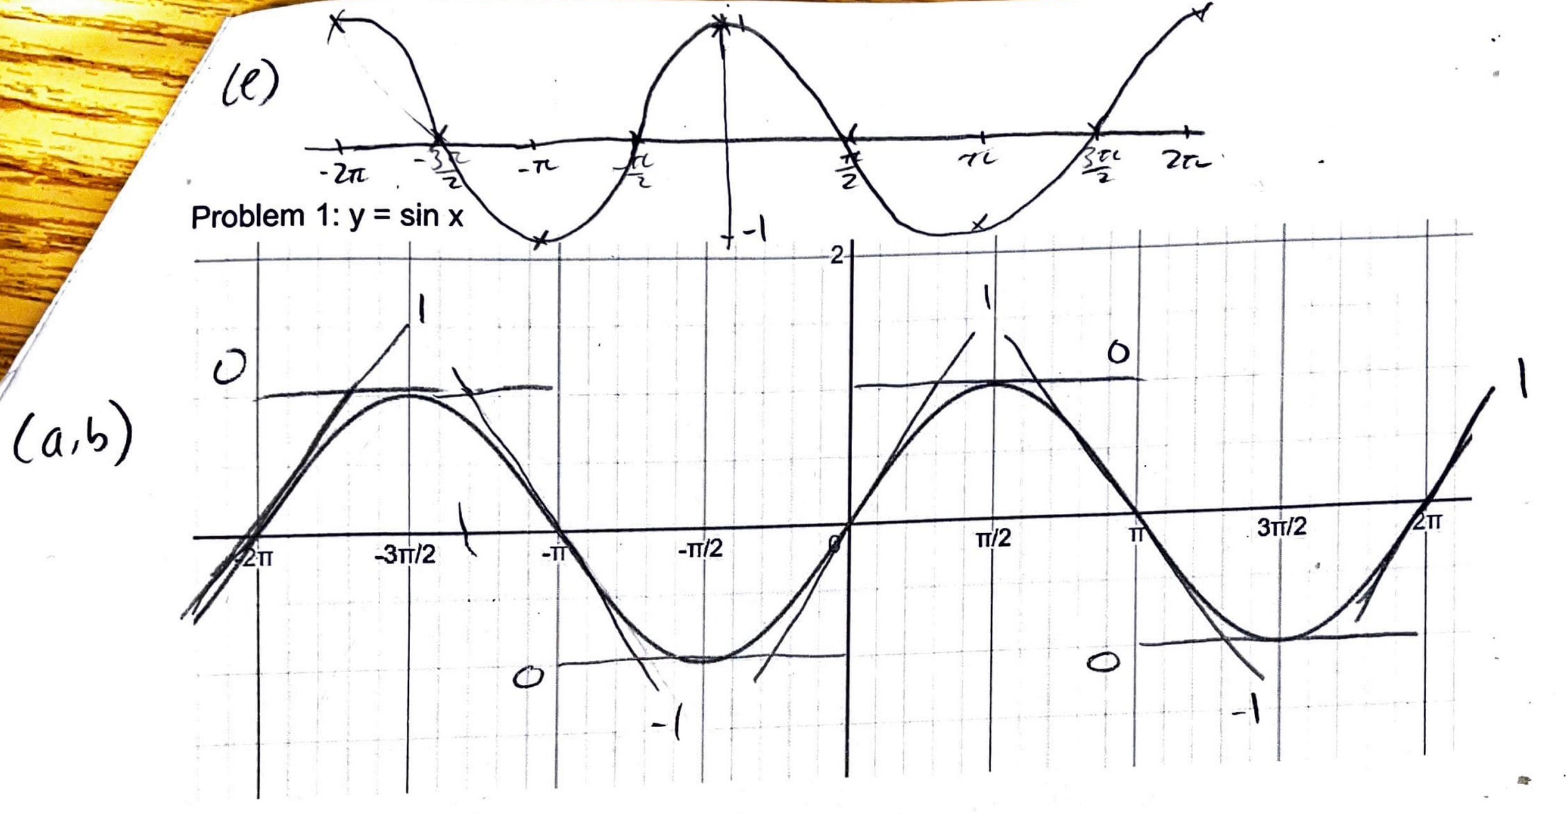
\includegraphics[width=.8\linewidth]{ps32q1abd.png}
\end{figure}

\item[(c)]
    \begin{align*}
        f'\left(0\right)&=\lim\limits_{h\to0}\frac{f\left(0+h\right)-f\left(0\right)}{h} \\
        &\approx\frac{f\left(0+0.0001\right)-f(0)}{0.0001} \\
        &=\frac{\sin(0.0001)-\sin0}{0.0001} \\
        &=0.9999999983\approx1\\
    \end{align*}
    Because $\sin x$ has a period of $2\pi$, its derivative will also have a period of $2\pi$. This suggests that $f'\left(2\pi\right)=f'\left(-2\pi\right)=1$.

\item[(e)]
    $y=\cos x$.

\end{itemize}

\section*{Problem 3}
\begin{itemize}
\item[(a)]
    \begin{align*}
        h(t)&=3\cos t-4\sin t \\
        h'(t)&=\diff{}{x}3\cos t-\diff{}{x}4\sin t \\
        \Aboxed{h'(t)&=-3\sin t-4\cos t}
    \end{align*}

\item[(b)]
    \begin{align*}
        y=f(t)&=2x+\frac{\sin x}{2} \\
        f'(t)&=\diff{}{t}2t+\diff{}{t}\left(\frac{1}{2}\sin t\right) \\
        &=2+\frac{\cos t}{2} \\
        \\
        f'\left(\frac{\pi}{6}\right)&=2+\frac{\cos\frac{\pi}{6}}{2} \\
        &=2+\frac{\sqrt{3}}{2}/2 \\
        &=\boxed{2+\frac{\sqrt{3}}{4}} \\
    \end{align*}

\item[(c)]
    \begin{align*}
        y=g(x)&=x^2+2\cos x \\
        g'(x)&=\diff{}{x}x^2+\diff{}{x}2\cos x\\
        &=2x+\left(-2\sin x\right) \\
        &=2x-2\sin x \\
        \\
        g'\left(\frac{\pi}{2}\right)&=2\cdot\frac{\pi}{2}-2\sin\frac{\pi}{2} \\
        &=\pi-2 \\
        \\
        y&=mx+c \\
        g\left(\frac{\pi}{2}\right)&=\left(\pi-2\right)\cdot\frac{\pi}{2}+c \\
        \left(\frac{\pi}{2}\right)^2+2\cos\frac{\pi}{2}&=\frac{\pi^2-2\pi}{2}+c \\
        \frac{\pi^2}{4}+2\cdot0&=\frac{\pi^2-2\pi}{2}+c \\
        \pi^2&=2\left(\pi^2-2\pi\right)+4c \\
        4c&=\pi^2-2\pi^2+4\pi \\
        c&=\frac{-\pi^2+4\pi}{4} \\
        c&=-\frac{\pi^{2}}{4}+\pi \\
        \Aboxed{y&=\left(\pi-2\right)x-\frac{\pi^2}{4}+\pi}
    \end{align*}

\item[(d)]
    \begin{align*}
        p(z)&=z^4+4^z+4\cos z-\sin\frac{\pi}{2} \\
        p'(z)&=\diff{}{z}z^4+\diff{}{z}4^z+\diff{}{z}4\cos z-\diff{}{z}\sin\frac{\pi}{2} \\
        &=4z^3+4^z\cdot\ln{4}+\left(-\sin z\right)-0 \\
        \Aboxed{p'(z)&=4z^3+4^z\cdot\ln{4}-4\sin z} \\
    \end{align*}

\item[(e)]
    \begin{align*}
        P(t)&=24+8\sin t \\
        P'(t)&=8\cdot\diff{}{t}\sin t \\
        P'(t)&=8\cos t
    \end{align*}
    2 decades have passed between January 1, 2010 and January 1, 2030.
    \begin{align*}
        P'(2)&=8\cos2 \\
        &\approx-3.32917\enspace\frac{\text{hundred animals}}{\text{decade}}
    \end{align*}
    as $P(t)$ is in hundreds of animals, $t$ is in decades. On January 1, 2030, the population of animals is decreasing at a rate of $3.32917$ hundred animals per decade.
\end{itemize}


\section*{Problem 5}
\begin{itemize}
\item[(c)]
    \begin{align*}
        f(x)&=4x^{25}\cos x \\
        f'(x)&=\diff{}{x}\left(4x^{25}\right)\cdot\cos x+4x^{25}\cdot\diff{}{x}\left(\cos x\right) \\
        f'(x)&=\left(4\cdot25\right)x^{24}\cdot\cos x+4x^{25}\cdot\left(-\sin x\right) \\
        \Aboxed{f'(x)&=100x^{24}\cos x-4x^{25}\sin x} \\
    \end{align*}

\item[(d)]
    \begin{align*}
        g(x)&=\cos\left(2021x\right)\cos\left(2022x\right)+\sin\left(2021x\right)\sin\left(2022x\right) \\
        &=\cos\left(2021x-2022x\right) \\
        &=\cos\left(-x\right) \\
        &=\cos x \\
        g'(x)&=\diff{}{x}\cos x \\
        \Aboxed{g'(x)&=-\sin x} \\
    \end{align*}

\item[(e)]
    \begin{align*}
        h(x)&=\sin\left(2022x\right)\cos\left(2021x\right)-\sin\left(2021x\right)\cos\left(2022x\right) \\
        &=\sin\left(2022x-2021x\right) \\
        &=\sin x \\
        h'(x)&=\diff{}{x}\sin x \\
        \Aboxed{h'(x)&=\cos x} \\
    \end{align*}
\end{itemize}


\section*{Problem 6}
    \begin{align*}
        y&=\frac{1}{\sin x+\cos x} \\
        \text{Let }f(x)&=\frac{1}{\sin x+\cos x} \\
        &=\left(\sin x+\cos x\right)^{-1} \\
        \\
        f'(x)&=\frac{-1}{\left(\sin x+\cos x\right)^2}\cdot\diff{}{x}\left(\sin x+\cos x\right) \\
        &=\frac{-\left(\cos x-\sin x\right)}{\left(\sin x+\cos x\right)^2} \\
        &=\frac{\sin x-\cos x}{\left(\sin x+\cos x\right)^2} \\
        \\
        f'(0)&=\frac{\sin0-\cos0}{\left(\sin0+\cos0\right)^2} \\
        &=\frac{0-1}{\left(0+1\right)^2} \\
        &=-1 \\
        \\
        y&=mx+c \\
        f(0)&=f'(0)x+c \\
        \frac{1}{\sin0+\cos0}&=-1\cdot0+c \\
        \frac{1}{0+1}&=c \\
        c&=1 \\
        \Aboxed{y&=-x+1} \\
    \end{align*}


\section*{Problem 9}
    \begin{align*}
        y&=\sec x-2\cos x \\
        \text{Let }f(x)&=\sec x-2\cos x \\
        &=\left(\cos x\right)^{-1}-2\cos x \\
        f'(x)&=\diff{}{x}\left(\cos x\right)^{-1}-\diff{}{x}\left(2\cos x\right) \\
        &=\frac{-1}{\left(\cos x\right)^2}\cdot\left(-\sin x\right)-2\left(-\sin x\right) \\
        &=\frac{\sin x}{\cos^2x}+2\sin x \\
        \\
        f'\left(\frac{\pi}{3}\right)&=\frac{\sin\frac{\pi}{3}}{\cos^2\frac{\pi}{3}}+2\sin\frac{\pi}{3} \\
        &=\frac{\sqrt{3}}{2}/\left(\frac{1}{2}\right)^2+2\cdot\frac{\sqrt{3}}{2} \\
        &=\frac{\sqrt{3}}{2}\cdot\frac{4}{1}+\sqrt{3} \\
        &=2\sqrt{3}+\sqrt{3} \\
        &=3\sqrt{3} \\
        \\
        y&=mx+c \\
        f\left(\frac{\pi}{3}\right)&=3\sqrt{3}\cdot\frac{\pi}{3}+c \\
        \left(\cos\frac{\pi}{3}\right)^{-1}-2\cos\frac{\pi}{3}&=\sqrt{3}\pi+c \\
        \left(\frac{1}{2}\right)^{-1}-2\cdot\frac{1}{2}&=\sqrt{3}\pi+c \\
        2-1&=\sqrt{3}\pi+c \\
        c&=1-\sqrt{3}\pi \\
        \\
        \Aboxed{y&=3\sqrt{3}x+1-\sqrt{3}\pi} \\
    \end{align*}


\section*{Problem 10}
\begin{align*}
    f\left(\frac{\pi}{3}\right)&=4 \\
    f'\left(\frac{\pi}{3}\right)&=-2 \\
    g\left(x\right)&=f\left(x\right)\cdot\sin x \\
    h\left(x\right)&=\frac{\cos x}{f\left(x\right)} \\
\end{align*}
\begin{itemize}
\item[(a)]
    \begin{align*}
        g'\left(x\right)&=\diff{}{x}\left(f\left(x\right)\cdot\sin x\right) \\
        &=f'\left(x\right)\cdot\sin x+f\left(x\right)\cdot\diff{}{x}\left(\sin x\right)\\
        &=f'\left(x\right)\cdot\sin x+f\left(x\right)\cdot\cos x\\
        g'\left(\frac{\pi}{3}\right)&=f'\left(\frac{\pi}{3}\right)\cdot\sin \frac{\pi}{3}+f\left(\frac{\pi}{3}\right)\cdot\cos\frac{\pi}{3} \\
        &=-2\cdot\frac{\sqrt{3}}{2}+4\cdot\frac{1}{2} \\
        &=-\sqrt{3}+2 \\
        &=\boxed{2-\sqrt{3}} \\
    \end{align*}

\item[(b)]
    \begin{align*}
        h'\left(x\right)&=\diff{}{x}\left(\frac{\cos x}{f\left(x\right)}\right) \\
        &=\frac{\diff{}{x}\left(\cos x\right)\cdot f\left(x\right)-\cos\left(x\right)\cdot\diff{f}{x}}{\left(f\left(x\right)\right)^2} \\
        &=\frac{-\sin x\cdot f\left(x\right)-\cos x\cdot f'\left(x\right)}{\left(f\left(x\right)\right)^2} \\
        h'\left(\frac{\pi}{3}\right)&=\frac{-\sin\frac{\pi}{3}\cdot f\left(\frac{\pi}{3}\right)-\cos\frac{\pi}{3}\cdot f'\left(\frac{\pi}{3}\right)}{\left(f\left(\frac{\pi}{3}\right)\right)^2} \\
        &=\frac{-\frac{\sqrt{3}}{2}\cdot4-\frac{1}{2}\left(-2\right)}{4^2} \\
        &=\frac{-2\sqrt{3}+1}{16} \\
        &=\boxed{\frac{1-2\sqrt{3}}{16}} \\
    \end{align*}
\end{itemize}


\section*{Problem 11}
\begin{itemize}
\item[(a)]
    \begin{align*}
        y&=5\cos\left(10x\right) \\
        \diff{y}{x}&=5\cdot\diff{}{x}\cos\left(10x\right) \\
        \diff{y}{x}&=5\cdot\left(-\sin\left(10x\right)\right)\cdot10 \\
        \Aboxed{\diff{y}{x}&=-50\sin\left(10x\right)} \\
    \end{align*}

\item[(b)]
    \begin{align*}
        f\left(x\right)&=\tan\left(\cos x\right) \\
        f'\left(x\right)&=\sec^2\left(\cos x\right)\cdot\left(-\sin x\right) \\
        \Aboxed{f'\left(x\right)&=-sec^2\left(\cos x\right)\sin x}
    \end{align*}

\item[(c)]
    \begin{align*}
        f\left(x\right)&=e^{x\cos x} \\
        f'\left(x\right)&=e^{x\cos x}\cdot\diff{}{x}\left(x\cos x\right) \\
        f'\left(x\right)&=e^{x\cos x}\cdot\left(1\cdot\cos x+x\cdot\left(-\sin x\right)\right) \\
        \Aboxed{f'\left(x\right)&=e^{x\cos x}\cdot\left(cos x-x\sin x\right)} \\
    \end{align*}

\item[(d)]
    \begin{align*}
        y&=\cot^2\left(\sin\theta\right) \\
        &=\frac{\left(\cos\left(\sin\theta\right)\right)^2}{\left(\sin\left(\sin\theta\right)\right)^2} \\
        \diff{y}{x}&=\diff{}{x}\left(\frac{\left(\cos\left(\sin\theta\right)\right)^2}{\left(\sin\left(\sin\theta\right)\right)^2}\right) \\
        &=\frac{\diff{}{x}\left(\cos\left(\sin\theta\right)\right)^2\cdot\sin^2\left(\sin\theta\right)-\diff{}{x}\left(\sin\left(\sin\theta\right)\right)^2\cdot\cos^2\left(\sin\theta\right)}{\left(\sin\left(\sin\theta\right)\right)^4} \\
        &=\frac{2\cos\left(\sin\theta\right)\cdot\diff{}{x}\left(\cos\left(\sin\theta\right)\right)\cdot\sin^2\left(\sin\theta\right)-2\sin\left(\sin\theta\right)\cdot\diff{}{x}\left(\sin\left(\sin\theta\right)\right)\cdot\cos^2\left(\sin\theta\right)}{\left(\sin\left(\sin\theta\right)\right)^4} \\
        &=\frac{2\cos\left(\sin\theta\right)\left(-\sin\left(\sin\theta\right)\cos\left(\theta\right)\right)\cdot\sin^{2}\left(\sin\theta\right)-2\sin\left(\sin\theta\right)\left(\cos\left(\sin\theta\right)\cos\left(\theta\right)\right)\cdot\cos^{2}\left(\sin\theta\right)}{\left(\sin\left(\sin\theta\right)\right)^{4}} \\
        &=\frac{-2\cos\left(\sin\theta\right)\sin\left(\sin\theta\right)\cos\left(\theta\right)\sin^{2}\left(\sin\theta\right)}{\left(\sin\left(\sin\theta\right)\right)^{4}}-\frac{2\sin\left(\sin\theta\right)\cos\left(\sin\theta\right)\cos\left(\theta\right)\cos^{2}\left(\sin\theta\right)}{\left(\sin\left(\sin\theta\right)\right)^{4}} \\
        &=\frac{-2\cos\left(\sin\theta\right)\cos\left(\theta\right)}{\sin\left(\sin\theta\right)}-\frac{2\left(\cos\left(\sin\theta\right)\right)^3\cos\left(\theta\right)}{\left(\sin\left(\sin\theta\right)\right)^{3}} \\
        \Aboxed{\diff{y}{x}&=-2\cot\left(\sin\theta\right)\cos\theta-2\cot^3\left(\sin\theta\right)\cos\theta} \\
    \end{align*}

\item[(e)]
    \begin{align*}
        \diff{\tan}{x}\left(x\right)&=\sec^2x \\
        \diff{\sec}{x}\left(x\right)&=\diff{}{x}\left(\cos x\right)^{-1}\\
        &=\frac{-1}{\left(-\cos x\right)^2}\cdot\left(-\sin x\right) \\
        &=\tan x\sec x \\
    \end{align*}
    \begin{align*}
        y&=\sec\left(2x\right)+\tan\left(2x\right) \\
        \diff{y}{x}&=\tan\left(2x\right)\sec\left(2x\right)\cdot2+\sec^2\left(2x\right)\cdot2 \\
        \Aboxed{\diff{y}{x}&=2\sec\left(2x\right)\left(\tan2x+\sec2x\right)} \\
    \end{align*}

\item[(f)]
    \begin{align*}
        y&=\cos\left(\frac{1-e^{2x}}{1+e^{2x}}\right) \\
        \diff{y}{x}&=-\sin\left(\frac{1-e^{2x}}{1+e^{2x}}\right)\cdot\diff{}{x}\left(\frac{1-e^{2x}}{1+e^{2x}}\right) \\
        &=-\sin\left(\frac{1-e^{2x}}{1+e^{2x}}\right)\cdot\frac{\diff{}{x}\left(1-e^{2x}\right)\cdot\left(1+e^{2x}\right)-\left(1-e^{2x}\right)\cdot\diff{}{x}\left(1+e^{2x}\right)}{\left(1+e^{2x}\right)^2} \\
        &=-\sin\left(\frac{1-e^{2x}}{1+e^{2x}}\right)\cdot\frac{-2e^{2x}\cdot\left(1+e^{2x}\right)-\left(1-e^{2x}\right)\cdot2e^{2x}}{\left(1+e^{2x}\right)^2} \\
        &=-\sin\left(\frac{1-e^{2x}}{1+e^{2x}}\right)\cdot\frac{-2e^{2x}-2e^{2x}\cdot e^{2x}-2e^{2x}+e^{2x}\cdot2e^{2x}}{\left(1+e^{2x}\right)^2} \\
        &=-\sin\left(\frac{1-e^{2x}}{1+e^{2x}}\right)\cdot\frac{-2e^{2x}-2e^{4x}-2e^{2x}+2e^{4x}}{\left(1+e^{2x}\right)^2} \\
        &=-\sin\left(\frac{1-e^{2x}}{1+e^{2x}}\right)\cdot\frac{-4e^{2x}}{\left(1+e^{2x}\right)^2} \\
        \Aboxed{\diff{y}{x}&=\sin\left(\frac{1-e^{2x}}{1+e^{2x}}\right)\cdot\frac{4e^{2x}}{\left(1+e^{2x}\right)^2}} \\
    \end{align*}

\item[(g)]
    \begin{align*}
        y&=\cos\left(\sqrt{\sin\left(\tan x\right)}\right) \\
        \diff{y}{x}&=-\sin\left(\sqrt{\sin\left(\tan x\right)}\right)\cdot\diff{}{x}\left(\sqrt{\sin\left(\tan x\right)}\right) \\
        &=-\sin\left(\sqrt{\sin\left(\tan x\right)}\right)\cdot\frac{1}{2\sqrt{\sin\left(\tan x\right)}}\cdot\diff{}{x}\left(\sin\left(\tan x\right)\right) \\
        &=-\sin\left(\sqrt{\sin\left(\tan x\right)}\right)\cdot\frac{1}{2\sqrt{\sin\left(\tan x\right)}}\cdot\cos\left(\tan x\right)\cdot\diff{}{x}\left(\tan x\right) \\
        \Aboxed{\diff{y}{x}&=-\frac{\sin\sqrt{\sin\left(\tan x\right)}}{2\sqrt{\sin\left(\tan x\right)}}\cdot\cos\left(\tan x\right)\cdot\sec^2x} \\
    \end{align*}

\item[(h)]
    \begin{align*}
        y&=\sin\left(\sin\left(\sin x\right)\right) \\
        \diff{y}{x}&=\cos\left(\sin\left(\sin x\right)\right)\cdot\diff{}{x}\left(\sin\left(\sin x\right)\right) \\
        &=\cos\left(\sin\left(\sin x\right)\right)\cdot\cos\left(\sin x\right)\cdot\diff{}{x}\sin x \\
        \Aboxed{\diff{y}{x}&=\cos\left(\sin\left(\sin x\right)\right)\cdot\cos\left(\sin x\right)\cdot\cos x} \\
    \end{align*}


\end{itemize}





\end{document}
